% !TEX TS-program = pdflatex
% !TEX encoding = UTF-8 Unicode

\documentclass[11pt]{report} % use larger type; default would be 10pt

\usepackage[utf8]{inputenc} % set input encoding (not needed with XeLaTeX)

%%% Examples of Article customizations
% These packages are optional, depending whether you want the features they provide.
% See the LaTeX Companion or other references for full information.

%%% PAGE DIMENSIONS
\usepackage{geometry} % to change the page dimensions
\geometry{a4paper} % or letterpaper (US) or a5paper or....
% \geometry{margin=2in} % for example, change the margins to 2 inches all round
% \geometry{landscape} % set up the page for landscape
%   read geometry.pdf for detailed page layout information

\usepackage{graphicx} % support the \includegraphics command and options

% \usepackage[parfill]{parskip} % Activate to begin paragraphs with an empty line rather than an indent

%%% PACKAGES
\usepackage{booktabs} % for much better looking tables
\usepackage{array} % for better arrays (eg matrices) in maths
\usepackage{paralist} % very flexible & customisable lists (eg. itemize/itemize, etc.)
\usepackage{verbatim} % adds environment for commenting out blocks of text & for better verbatim
\usepackage{subfig} % make it possible to include more than one captioned figure/table in a single float
% These packages are all incorporated in the memoir class to one degree or another...

%%% HEADERS & FOOTERS
\usepackage{fancyhdr} % This should be set AFTER setting up the page geometry
\pagestyle{fancy} % options: empty , plain , fancy
\renewcommand{\headrulewidth}{0pt} % customise the layout...
\lhead{}\chead{Use Case Diagrams}\rhead{}
\lfoot{}\cfoot{\thepage}\rfoot{}

%%% SECTION TITLE APPEARANCE
\usepackage{sectsty}
\allsectionsfont{\sffamily\mdseries\upshape} % (See the fntguide.pdf for font help)
% (This matches ConTeXt defaults)

%%% ToC (table of contents) APPEARANCE
\usepackage[nottoc,notlof,notlot]{tocbibind} % Put the bibliography in the ToC
\usepackage[titles,subfigure]{tocloft} % Alter the style of the Table of Contents
\usepackage{graphicx}

\renewcommand{\cftsecfont}{\rmfamily\mdseries\upshape}
\renewcommand{\cftsecpagefont}{\rmfamily\mdseries\upshape} % No bold!

%%% END Article customizations

%%% The "real" document content comes below...

\title{Software Engineering Project - Links \\Use Case Diagrams}
\author{Abhijith Madhav, Arjun S Bharadwaj}
%\date{} % Activate to display a given date or no date (if empty),
         % otherwise the current date is printed 

\begin{document}
\maketitle
\section*{Abbreviations}
\begin{enumerate}
	\item
		LAU – Links API user
	\item
		LU – Links user
	\item
		L - Links
\end{enumerate}

\maketitle
\section*{Use case diagram}
Below is the use case diagram of “Links” depicting two actors.
\begin{figure}[h]
\centering
        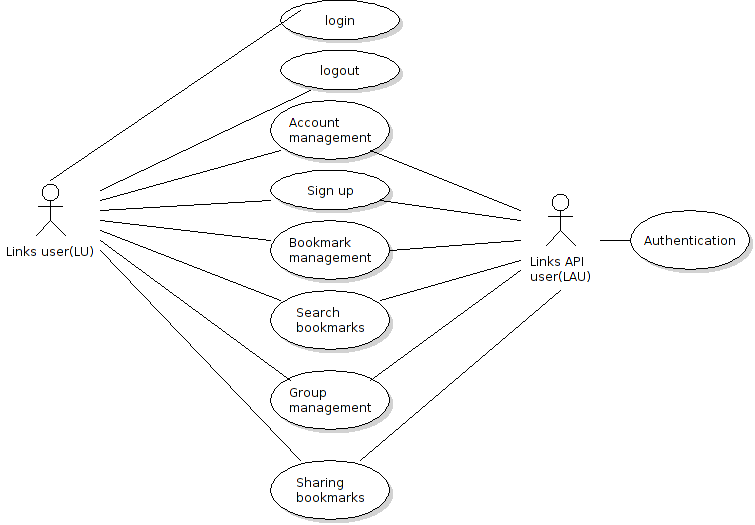
\includegraphics[width=\textwidth]{usecase}
    \caption{{Links - Use Case Diagram}.}
    \label{fig:Use Case Diagram}
\end{figure}


\maketitle
\section*{User Cases}
This section wil list all the Use cases related to the actors.
\begin{enumerate}

\item
	Login
		\begin{enumerate}
			\item
				Sequence 1
					\begin{enumerate}
						\item
							LU: Clicks on login link.
						\item
							L: Presents the login page.
						\item
							LU: Enters user name and password.
						\item
							L: Displays the message that the user has been logged in.
					\end{enumerate}
			\item
				Sequence 2: At step iv of Sequence 1
					\begin{enumerate}
						\item
							L: Display message that the authentication details are incorrect.						
					\end{enumerate}
		\end{enumerate}

\item
	Logout
		\begin{enumerate}
			\item
				Sequence 1
					\begin{enumerate}
						\item
							LU: Clicks on logout link.
						\item
							Links: Displays message that the user has been logged out.			
					\end{enumerate}
		\end{enumerate}

\item
	Authentication
		\begin{enumerate}
			\item
				Sequence 1
					\begin{enumerate}
						\item
							LUA: Requests for an authenticated session.
						\item
							L: Asks for authentication details from the LU.
						\item
							LU: Provides username and password.
						\item
							L: Provides the LUA with an authenticated session.
					\end{enumerate}
			\item
				Sequence 2: At step iv of Sequence 1
					\begin{enumerate}
						\item
							L: Indicates that authentication details are incorrect					
					\end{enumerate}
		\end{enumerate}

\item
	Sign up
		\begin{enumerate}
			\item
				Sequence 1
					\begin{enumerate}
						\item
							LU/LAU: Requests a “Sign up” operation.
						\item
							L: Asks for details regarding the user.
						\item
							LU/LAU: Provides relevant details.
						\item
							L: Confirms account creation pending email verification.
						\item
							LU: Verifies through email.
						\item
							L: Confirms account creation.

					\end{enumerate}
			\item
				Sequence 2: At step iv of Sequence 1
					\begin{enumerate}
						\item
							L: Points out inconsistencies in entry of user details.		
					\end{enumerate}
		\end{enumerate}

\item
	Account management
		\begin{enumerate}
			\item
				Sequence 1
					\begin{enumerate}
						\item
							LU/LAU: Requests a “Modify account” operation after logging in or after authentication.
						\item
							L: Return account details.
						\item
							LU/LAU: Modifies details and requests an “Update” operation.
						\item
							L: Confirm update of account details.						

					\end{enumerate}			
		\end{enumerate}

\item
	Bookmark Management
		\begin{enumerate}
			\item
				Sequence 1
					\begin{enumerate}
						\item
							LAU/LU: Specifies an “Add Bookmark” operation after authentication/logging in.
						\item
							L: Asks for new bookmark details.
						\item
							LU/LAU: Populate the data and submits.
						\item
							L: Confirms addition of new links.
					\end{enumerate}
			\item
				Sequence 2
					\begin{enumerate}
						\item
							LAU/LU: Specifies an “Update Bookmark” operation along with details of an associated bookmark after authentication/logging in.
						\item
							L: Presents existing data about the bookmark.
						\item
							LU: Modifies details and submits.
						\item
							L: Confirms update.
					\end{enumerate}
			\item
				Sequence 3
					\begin{enumerate}
						\item
							LU: Specifies a “Delete Bookmark” operation along with details of an associated bookmark after authentication/logging in.
						\item
							L: Confirms deletion of bookmark.
					\end{enumerate}
		\end{enumerate}

\item
	Search bookmarks
		\begin{enumerate}
			\item
				Sequence 1
					\begin{enumerate}
						\item
							LU/LAU: Specifies a “Search” operation along with search keywords.
						\item
							L: Presents bookmarks satisfying the search criteria.				
					\end{enumerate}			
		\end{enumerate}


\item
	Share bookmarks
		\begin{enumerate}
			\item
				Sequence 1
					\begin{enumerate}
						\item
							LU/LUA: Specifies “Share bookmarks operation” after authentication/logging in.
						\item
							L: Asks for list of bookmarks to share and for medium to share through – email, Facebook, Twitter, groups.
						\item
							LU: Specifies list of bookmarks and a sharing medium.
						\item
							L: Shares bookmarks through the selected medium.
					\end{enumerate}
		\end{enumerate}

\item
	Group management
		\begin{enumerate}
			\item
				Sequence 1
					\begin{enumerate}
						\item
							LU/LUA: Requests a “Create Group” operation after authentication/logging in.
						\item
							L: Asks for relevant details.
						\item
							LU/LUA: Provides relevant details.
						\item
							L: Confirms creation of group.
					\end{enumerate}

			\item
				Sequence 2
					\begin{enumerate}
						\item
							LU/LUA: Requests a “Remove from group” operation for a particular user after logging in / authentication.
						\item
							L: Confirms removal of member from the group.
					\end{enumerate}

			\item
				Sequence 3
					\begin{enumerate}
						\item
							LU/LUA: Requests a “Add to group” operation after logging in / authentication.
						\item
							L: Asks for user name and group.
						\item
							LU/LUA: Submits information.
						\item
							L: Confirms addition to group.
					\end{enumerate}

			\item
				Sequence 4
					\begin{enumerate}
						\item
							LU/LUA: Requests a “Join to group” operation after authentication/logging in.
						\item
							L: Asks for group name.
						\item
							LU/LUA: Submits information.
						\item
							L: Confirms subscription.
					\end{enumerate}

			\item
				Sequence 5
					\begin{enumerate}
						\item
							LU/LUA: Requests for an “Unjoin group” operation after logging in / authentication.
						\item
							L: Asks for group name.
						\item
							LU/LUA: Submits information.
						\item
							L: Confirms removal from specified group.
					\end{enumerate}

		\end{enumerate}
\end{enumerate}
\end{document}
